\documentclass[11pt]{article}
\usepackage[margin=1in]{geometry}
\usepackage{tikz}
\usepackage{pgfplots}
\usetikzlibrary{shapes,arrows,positioning,fit,backgrounds,matrix}
\usepackage{booktabs}
\usepackage{multirow}
\usepackage{amsmath}
\usepackage{xcolor}
\usepackage{listings}
\usepackage{hyperref}

\definecolor{codegreen}{rgb}{0,0.6,0}
\definecolor{codegray}{rgb}{0.5,0.5,0.5}
\definecolor{codepurple}{rgb}{0.58,0,0.82}
\definecolor{backcolour}{rgb}{0.95,0.95,0.92}

\lstdefinestyle{mystyle}{
    backgroundcolor=\color{backcolour},
    commentstyle=\color{codegreen},
    keywordstyle=\color{magenta},
    numberstyle=\tiny\color{codegray},
    stringstyle=\color{codepurple},
    basicstyle=\ttfamily\footnotesize,
    breakatwhitespace=false,
    breaklines=true,
    captionpos=b,
    keepspaces=true,
    numbers=left,
    numbersep=5pt,
    showspaces=false,
    showstringspaces=false,
    showtabs=false,
    tabsize=2
}

\lstset{style=mystyle}

\title{Comprehensive Summary: Diabetic Retinopathy Feature Extraction Pipeline}
\author{Medical Image Processing System}
\date{\today}

\begin{document}

\maketitle

\begin{abstract}
This document provides a comprehensive technical summary of the diabetic retinopathy feature extraction pipeline, including the nature of extracted features, derived statistics, target variables, and complete data processing workflow. The system employs multi-modal feature extraction combining traditional computer vision with deep learning approaches for early detection of diabetic retinopathy.
\end{abstract}

\tableofcontents

\section{Introduction}

Diabetic retinopathy (DR) is a leading cause of blindness worldwide. This automated feature extraction pipeline processes retinal images to extract comprehensive features that characterize various pathological manifestations of DR. The system integrates multiple feature extraction heads targeting specific retinal structures and abnormalities.

\section{Overall Pipeline Architecture}

\begin{figure}[h!]
\centering
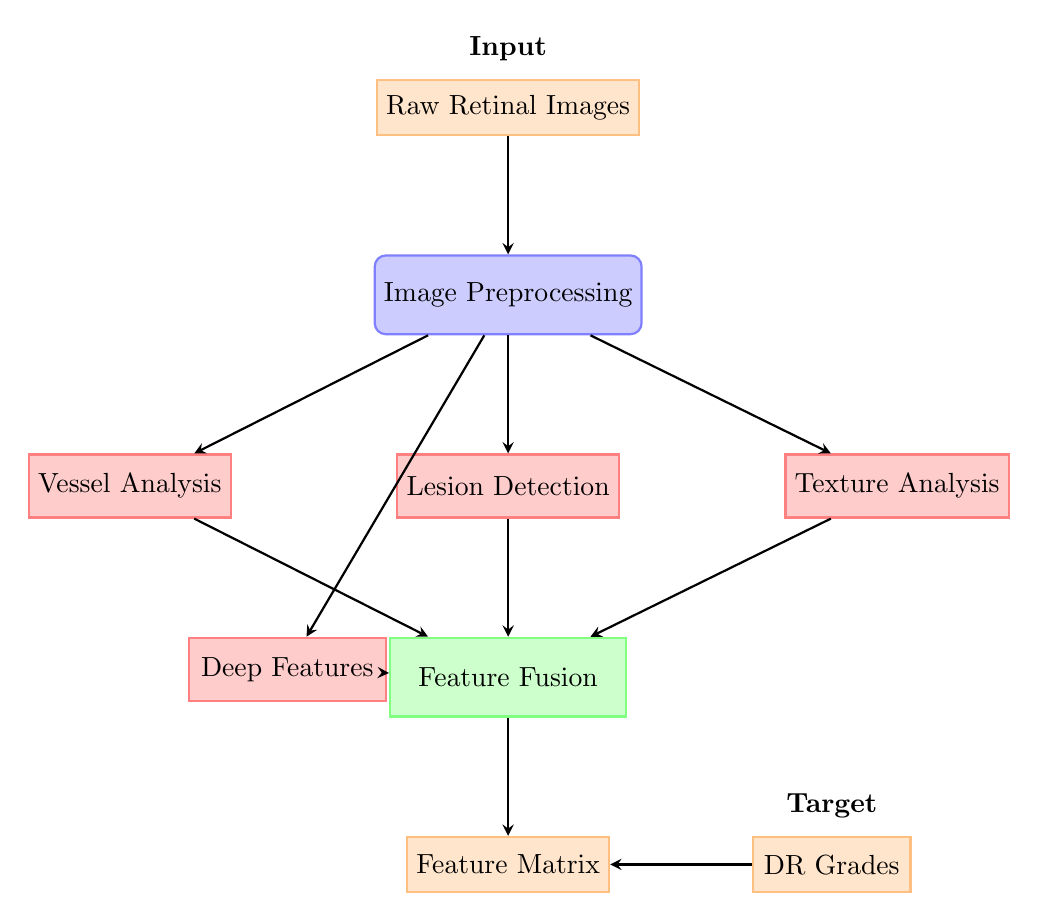
\begin{tikzpicture}[
    node distance=1.5cm and 0.8cm,
    stage/.style={rectangle, draw=blue!50, fill=blue!20, thick, minimum width=3cm, minimum height=1cm, text centered, rounded corners},
    process/.style={rectangle, draw=green!50, fill=green!20, thick, minimum width=3cm, minimum height=1cm, text centered},
    feature/.style={rectangle, draw=red!50, fill=red!20, thick, minimum width=2.5cm, minimum height=0.8cm, text centered},
    data/.style={rectangle, draw=orange!50, fill=orange!20, thick, minimum width=2cm, minimum height=0.7cm, text centered},
    arrow/.style={->, >=stealth, thick}
]

% Nodes
\node (input) [data] {Raw Retinal Images};
\node (preprocess) [stage, below=of input] {Image Preprocessing};
\node (vessel) [feature, below left=of preprocess, xshift=-1cm] {Vessel Analysis};
\node (lesions) [feature, below=of preprocess] {Lesion Detection};
\node (texture) [feature, below right=of preprocess, xshift=1cm] {Texture Analysis};
\node (deep) [feature, below=of vessel, xshift=2cm] {Deep Features};
\node (fusion) [process, below=of lesions] {Feature Fusion};
\node (output) [data, below=of fusion] {Feature Matrix};
\node (target) [data, right=of output, xshift=1cm] {DR Grades};

% Arrows
\draw [arrow] (input) -- (preprocess);
\draw [arrow] (preprocess) -- (vessel);
\draw [arrow] (preprocess) -- (lesions);
\draw [arrow] (preprocess) -- (texture);
\draw [arrow] (preprocess) -- (deep);
\draw [arrow] (vessel) -- (fusion);
\draw [arrow] (lesions) -- (fusion);
\draw [arrow] (texture) -- (fusion);
\draw [arrow] (deep) -- (fusion);
\draw [arrow] (fusion) -- (output);
\draw [arrow] (target) -- (output);

% Labels
\node [above=0.1cm of input] {\textbf{Input}};
\node [above=0.1cm of target] {\textbf{Target}};

\end{tikzpicture}
\caption{Overall Feature Extraction Pipeline Architecture}
\label{fig:pipeline}
\end{figure}

\section{Feature Extraction Categories}

\subsection{Vessel Structure Analysis}
\begin{table}[h!]
\centering
\begin{tabular}{p{0.25\textwidth}p{0.3\textwidth}p{0.35\textwidth}}
\toprule
\textbf{Feature Type} & \textbf{Extraction Method} & \textbf{Derived Statistics} \\
\midrule
Blood Vessel Density & Frangi/Sato filter multi-scale enhancement & Mean response, Standard deviation, Maximum response, 95th percentile, Entropy \\
Vessel Tortuosity & Skeletonization and curvature analysis & Tortuosity index, Branching points, Vessel length distribution \\
Vessel Caliber & Morphological operations & Mean vessel width, Width variance, Arteriovenous ratio \\
\bottomrule
\end{tabular}
\caption{Vessel Structure Feature Extraction}
\end{table}

\subsection{Lesion Detection and Characterization}
\begin{table}[h!]
\centering
\begin{tabular}{p{0.25\textwidth}p{0.3\textwidth}p{0.35\textwidth}}
\toprule
\textbf{Lesion Type} & \textbf{Detection Method} & \textbf{Quantitative Measures} \\
\midrule
Microaneurysms & Difference of Gaussians + circularity filter & Count, Mean area, Eccentricity, Total lesion area ratio \\
Hemorrhages & Low-intensity region analysis + shape filtering & Count, Mean area, Eccentricity, Intensity statistics, Area ratio \\
Exudates & High-intensity region analysis + texture filtering & Count, Mean area, Eccentricity, Mean intensity, Area ratio \\
Cotton Wool Spots & Fuzzy boundary detection & Count, Size distribution, Location relative to optic disc \\
\bottomrule
\end{tabular}
\caption{Lesion-based Feature Extraction}
\end{table}

\subsection{Anatomical Structure Analysis}
\begin{table}[h!]
\centering
\begin{tabular}{p{0.25\textwidth}p{0.3\textwidth}p{0.35\textwidth}}
\toprule
\textbf{Structure} & \textbf{Localization Method} & \textbf{Extracted Features} \\
\midrule
Optic Disc & Brightness-based segmentation + circular Hough transform & Area, Eccentricity, Solidity, Mean intensity, Size ratio \\
Macula & Central dark region analysis & Mean intensity, Standard deviation, Minimum intensity, Entropy, Area ratio \\
Fovea & Central avascular zone detection & Central reflex presence, Pigment distribution, Symmetry \\
\bottomrule
\end{tabular}
\caption{Anatomical Structure Feature Extraction}
\end{table}

\section{Statistical Feature Derivation}

\begin{figure}[h!]
\centering
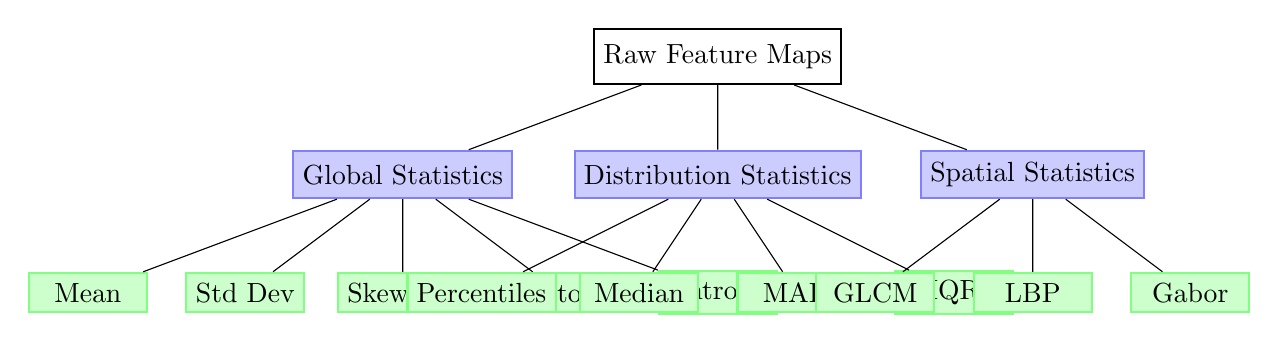
\begin{tikzpicture}[
    level 1/.style={sibling distance=4cm},
    level 2/.style={sibling distance=2cm},
    level 3/.style={sibling distance=1.5cm},
    feature/.style={rectangle, draw=black, thick, minimum width=2cm, minimum height=0.7cm, text centered},
    stat/.style={rectangle, draw=blue!50, fill=blue!20, thick, minimum width=1.8cm, minimum height=0.6cm, text centered},
    leaf/.style={rectangle, draw=green!50, fill=green!20, thick, minimum width=1.5cm, minimum height=0.5cm, text centered}
]

% Root
\node [feature] {Raw Feature Maps}
    child { node [stat] {Global Statistics}
        child { node [leaf] {Mean} }
        child { node [leaf] {Std Dev} }
        child { node [leaf] {Skewness} }
        child { node [leaf] {Kurtosis} }
        child { node [leaf] {Entropy} }
    }
    child { node [stat] {Distribution Statistics}
        child { node [leaf] {Percentiles} }
        child { node [leaf] {Median} }
        child { node [leaf] {MAD} }
        child { node [leaf] {IQR} }
    }
    child { node [stat] {Spatial Statistics}
        child { node [leaf] {GLCM} }
        child { node [leaf] {LBP} }
        child { node [leaf] {Gabor} }
    };

\end{tikzpicture}
\caption{Statistical Feature Derivation Hierarchy}
\label{fig:stats_hierarchy}
\end{figure}

\subsection{Global Image Statistics}
\begin{equation}
\begin{aligned}
\text{Mean Intensity} &= \frac{1}{N}\sum_{i=1}^{N} I_i \\
\text{Standard Deviation} &= \sqrt{\frac{1}{N}\sum_{i=1}^{N} (I_i - \mu)^2} \\
\text{Skewness} &= \frac{\frac{1}{N}\sum_{i=1}^{N} (I_i - \mu)^3}{\sigma^3} \\
\text{Kurtosis} &= \frac{\frac{1}{N}\sum_{i=1}^{N} (I_i - \mu)^4}{\sigma^4} - 3 \\
\text{Entropy} &= -\sum_{k=1}^{K} p_k \log_2 p_k
\end{aligned}
\end{equation}

\subsection{Regional Feature Statistics}
For each detected region $R$ (vessels, lesions, etc.):
\begin{equation}
\begin{aligned}
\text{Region Count} &= N_R \\
\text{Mean Area} &= \frac{1}{N_R}\sum_{i=1}^{N_R} A_i \\
\text{Area Ratio} &= \frac{\sum_{i=1}^{N_R} A_i}{A_{\text{total}}} \\
\text{Eccentricity} &= \frac{1}{N_R}\sum_{i=1}^{N_R} e_i
\end{aligned}
\end{equation}

\section{Target Variable Specification}

\subsection{Diabetic Retinopathy Grading Scale}
\begin{table}[h!]
\centering
\begin{tabular}{p{0.15\textwidth}p{0.2\textwidth}p{0.55\textwidth}}
\toprule
\textbf{Grade} & \textbf{Label} & \textbf{Clinical Description} \\
\midrule
0 & No DR & No apparent retinopathy \\
1 & Mild NPDR & Microaneurysms only \\
2 & Moderate NPDR & More than just microaneurysms but less than severe NPDR \\
3 & Severe NPDR & Any of the following: 20+ intraretinal hemorrhages in 4 quadrants, definite venous beading in 2+ quadrants, prominent IRMA in 1+ quadrant, and no signs of PDR \\
4 & PDR & One or more of: vitreous/preretinal hemorrhage, neovascularization, or tractional retinal detachment \\
\bottomrule
\end{tabular}
\caption{Diabetic Retinopathy International Clinical Classification}
\end{table}

\section{Complete Feature Matrix Structure}

\begin{figure}[h!]
\centering
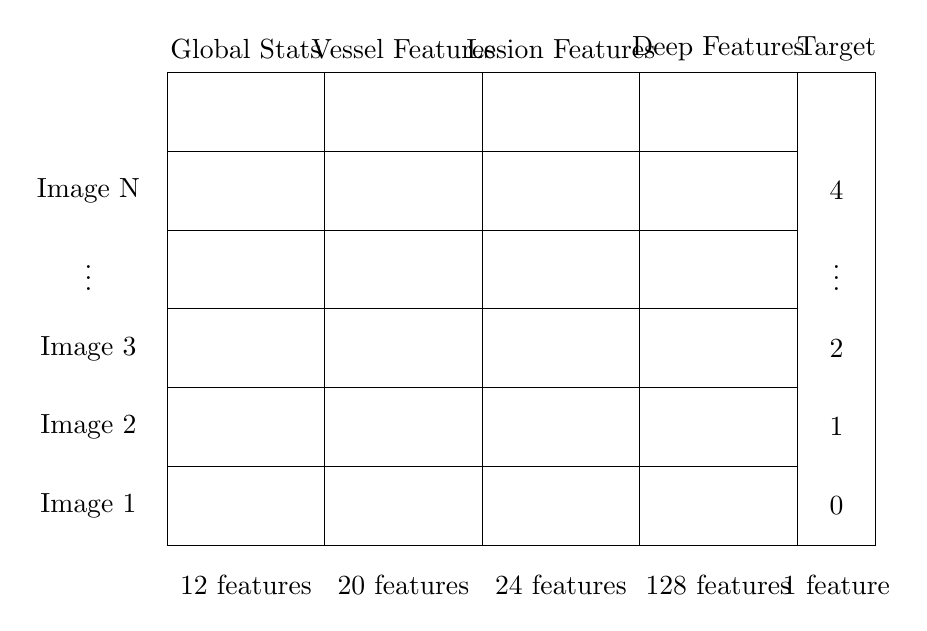
\begin{tikzpicture}

% Feature matrix
\draw (0,0) rectangle (8,6);
\draw (2,0) -- (2,6);
\draw (4,0) -- (4,6);
\draw (6,0) -- (6,6);

\draw (0,1) -- (8,1);
\draw (0,2) -- (8,2);
\draw (0,3) -- (8,3);
\draw (0,4) -- (8,4);
\draw (0,5) -- (8,5);

% Column labels
\node at (1,6.3) {Global Stats};
\node at (3,6.3) {Vessel Features};
\node at (5,6.3) {Lesion Features};
\node at (7,6.3) {Deep Features};

% Row labels
\node at (-1,0.5) {Image 1};
\node at (-1,1.5) {Image 2};
\node at (-1,2.5) {Image 3};
\node at (-1,3.5) {\vdots};
\node at (-1,4.5) {Image N};

% Target column
\draw (8,0) rectangle (9,6);
\node at (8.5,6.3) {Target};
\node at (8.5,0.5) {0};
\node at (8.5,1.5) {1};
\node at (8.5,2.5) {2};
\node at (8.5,3.5) {\vdots};
\node at (8.5,4.5) {4};

% Feature counts
\node at (1, -0.5) {12 features};
\node at (3, -0.5) {20 features};
\node at (5, -0.5) {24 features};
\node at (7, -0.5) {128 features};
\node at (8.5, -0.5) {1 feature};

\end{tikzpicture}
\caption{Feature Matrix Structure (N images × 184 features + target)}
\label{fig:feature_matrix}
\end{figure}

\section{Data Processing Pipeline Details}

\subsection{Input Data Specifications}
\begin{table}[h!]
\centering
\begin{tabular}{p{0.3\textwidth}p{0.65\textwidth}}
\toprule
\textbf{Parameter} & \textbf{Specification} \\
\midrule
Supported Formats & PNG, JPEG, TIFF, BMP \\
Input Resolution & Variable (auto-resized to 512×512) \\
Color Space & RGB (converted from BGR if needed) \\
Preprocessing & CLAHE contrast enhancement, Gaussian smoothing \\
Data Organization & Grade-based folder structure (grade\_0, grade\_1, etc.) \\
\bottomrule
\end{tabular}
\caption{Input Data Specifications}
\end{table}

\subsection{Feature Extraction Computational Profile}
\begin{table}[h!]
\centering
\begin{tabular}{p{0.3\textwidth}p{0.25\textwidth}p{0.4\textwidth}}
\toprule
\textbf{Feature Category} & \textbf{Processing Time} & \textbf{Memory Requirements} \\
\midrule
Global Statistics & 10-50 ms/image & Low (10-50 MB) \\
Vessel Analysis & 100-500 ms/image & Medium (100-200 MB) \\
Lesion Detection & 200-800 ms/image & Medium (150-300 MB) \\
Texture Analysis & 50-200 ms/image & Low-Medium (50-150 MB) \\
Deep Features & 500-2000 ms/image & High (500-1000 MB) \\
Complete Pipeline & 1-4 seconds/image & 800-2000 MB peak \\
\bottomrule
\end{tabular}
\caption{Computational Requirements per Image}
\end{table}

\section{Quality Control and Validation}

\subsection{Feature Quality Metrics}
\begin{itemize}
\item \textbf{Completeness Rate}: Percentage of successfully extracted features per image
\item \textbf{Feature Variance}: Measures discriminative power across classes
\item \textbf{Correlation Analysis}: Identifies redundant features
\item \textbf{Null Value Handling}: Strategies for missing feature values
\end{itemize}

\subsection{Validation Framework}
\begin{table}[h!]
\centering
\begin{tabular}{p{0.25\textwidth}p{0.7\textwidth}}
\toprule
\textbf{Validation Type} & \textbf{Implementation} \\
\midrule
Cross-validation & Stratified k-fold (k=5/10) preserving class distribution \\
Train-Test Split & 70-30 or 80-20 split with stratification \\
Feature Scaling & StandardScaler or MinMaxScaler applied to training data \\
Class Imbalance & SMOTE oversampling or class weighting in models \\
Performance Metrics & Accuracy, Precision, Recall, F1-score, ROC-AUC \\
\bottomrule
\end{tabular}
\caption{Model Validation Framework}
\end{table}

\section{Implementation Details}

\subsection{Software Dependencies}
\begin{lstlisting}[language=Python, caption=Core Dependencies]
# Computer Vision & Image Processing
opencv-python>=4.5.0
scikit-image>=0.18.0
scipy>=1.7.0
numpy>=1.21.0

# Machine Learning & Deep Learning
scikit-learn>=1.0.0
torch>=1.9.0
torchvision>=0.10.0

# Data Handling & Utilities
pandas>=1.3.0
tqdm>=4.60.0
psutil>=5.8.0
\end{lstlisting}

\subsection{Key Configuration Parameters}
\begin{lstlisting}[language=Python, caption=Configuration Parameters]
# Image Processing
IMAGE_SIZE = (512, 512)
CLAHE_CLIP_LIMIT = 2.0
GAUSSIAN_SIGMA = 1.0

# Feature Extraction
VESSEL_SCALES = [1, 2, 3, 4]
LESION_SIZE_RANGE = (50, 10000)
GLCM_DISTANCES = [1, 3]
GLCM_ANGLES = [0, np.pi/4, np.pi/2]

# Memory Management
MAX_MEMORY_MB = 6000
BATCH_SIZE = 10
FEATURE_DIMENSION_LIMIT = 2048
\end{lstlisting}

\section{Conclusion}

This comprehensive feature extraction pipeline provides a robust foundation for diabetic retinopathy detection and classification. The multi-modal approach combining traditional image analysis with deep learning features captures both localized pathological changes and global retinal characteristics. The extracted feature set enables both clinical interpretation and high-performance machine learning model development for early DR detection.

\end{document}
